
%%%%%%%%%%%%%%%%%%%%%%%%%%%%%%%%%%%%%%%%%%%%%%%%%%%%%%%%%%
%%
%% This is the "PREAMBLE". Here we define the type of document and load in any packages we might want. You can also set parameters %% % and create your own short-hand here.
%%
%%%%%%%%%%%%%%%%%%%%%%%%%%%%%%%%%%%%%%%%%%%%%%%%%%%%%%%%%%

 \documentclass[9pt]{article}

 \def\solutions{0}


 \usepackage{amsmath}
 \usepackage{amssymb}
 \usepackage{graphicx}    % needed for including graphics e.g. EPS, PS \usepackage{tikz}
 \usepackage{tikz}
 \usepackage{tikzsymbols}
 \usepackage{relsize}
 \usetikzlibrary{patterns,decorations.pathreplacing,shapes,arrows}
 \usetikzlibrary{calc, matrix, arrows.meta}
 \usepackage{algorithm2e}
 \topmargin -2.5cm        % read Lamport p.163
 \oddsidemargin -0.04cm   % read Lamport p.163
 \evensidemargin -0.04cm  % same as oddsidemargin but for left-hand pages
 \textwidth 16.59cm
 \textheight 25.94cm
% \pagestyle{empty}        % Uncomment if don't want page numbers
 \pagenumbering{gobble}
 \parskip 7.2pt           % sets spacing between paragraphs
 %\renewcommand{\baselinestretch}{1.5} 	% Uncomment for 1.5 spacing between lines
 \parindent 0pt		  % sets leading space for paragraphs

% No date in header
\date{}

\usepackage{hyperref}
\hypersetup{
    colorlinks=true,
    linkcolor=blue,
    filecolor=magenta,
    urlcolor=cyan,
}
\usepackage{amsthm}
\usepackage{fancyhdr}
\pagestyle{fancy}
\setlength{\headsep}{36pt}

\usepackage{hyperref}

\newcommand{\lp}{\left(}
\newcommand{\rp}{\right)}
\newcommand{\lb}{\left[}
\newcommand{\rb}{\right]}
\newcommand{\ls}{\left\{}
\newcommand{\rs}{\right\}}
\newcommand{\lbar}{\left|}
\newcommand{\rbar}{\right|}
\newcommand{\ld}{\left.}
\newcommand{\rd}{\right.}

\newcommand{\myexists}{\exists \hspace{.3mm}}

\newcommand{\hs}{\hspace{.75mm}}
\newcommand{\bs}{\hspace{-.75mm}}
\newcommand{\nin}{\noindent}

\newcommand{\fx}{f\bs\left( x \right)}
\newcommand{\gx}{g\bs\left( x \right)}
\newcommand{\qx}{q\bs\left( x \right)}

\newcommand{\nn}{\nonumber}

\newcommand{\vfive}{\vspace{5mm}}
\newcommand{\vthree}{\vspace{3mm}}

\newcommand{\fof}[1]{f\lp #1\rp}
\newcommand{\gof}[1]{g\lp #1\rp}
\newcommand{\qof}[1]{q\lp #1\rp}

\newcommand{\myp}[1]{\left( #1 \right)}
\newcommand{\myb}[1]{\left[ #1 \right]}
\newcommand{\mys}[1]{\left\{ #1 \right\}}
\newcommand{\myab}[1]{\left| #1 \right|}

\newcommand{\myj}{_j}
\newcommand{\myjp}{_{j+1}}
\newcommand{\myjm}{_{j-1}}

\newcommand{\f}[1]{f\hspace{-1mm}\left( #1 \right)}
\newcommand{\fp}[1]{f'\hspace{-1mm}\left( #1 \right)}
\newcommand{\g}[1]{g\hspace{-1mm}\left( #1 \right)}
\newcommand{\gp}[1]{g'\hspace{-1mm}\left( #1 \right)}
\newcommand{\q}[1]{q\hspace{-1mm}\left( #1 \right)}
\newcommand{\qp}[1]{q'\hspace{-1mm}\left( #1 \right)}
\newcommand{\Px}[1]{P\hspace{-1mm}\left( x_{#1} \right)}
\newcommand{\Qx}[1]{Q\hspace{-1mm}\left( x_{#1} \right)}

\newcommand{\tten}[1]{\times 10^{#1}}

\newcommand{\aij}[1]{a_{#1}}
\newcommand{\bij}[1]{b_{#1}}
\newcommand{\rij}[1]{r_{#1}}

\newcommand{\R}[1]{\mathbb{R}^{#1}}

\newcommand{\ith}{i^{\textrm{th}}}
\newcommand{\jth}{i^{\textrm{th}}}
\newcommand{\kth}{i^{\textrm{th}}}

\newcommand{\inv}[1]{{#1}^{-1}}

\newcommand{\bx}{\mathbf{x}}
\newcommand{\bv}{\mathbf{v}}
\newcommand{\bw}{\mathbf{w}}
\newcommand{\by}{\mathbf{y}}
\newcommand{\bb}{\mathbf{b}}
\newcommand{\be}{\mathbf{e}}
\newcommand{\br}{\mathbf{r}}
\newcommand{\xhat}{\hat{\mathbf{x}}}

\newcommand{\beq}{\begin{eqnarray}}
\newcommand{\eeq}{\end{eqnarray}}

\newcommand{\ben}{\begin{enumerate}}
\newcommand{\een}{\end{enumerate}}

\newcommand{\bsq}{\mathsmaller{\blacksquare}}

\newcommand{\iter}[1]{^{\myp{#1}}}

% matrix macro
\newcommand{\mymat}[1]{
\left[
\begin{array}{rrrrrrrrrrrrrrrrrrrrrrrrrrrrrrrrrrrrrrr}
#1
\end{array}
\right]
}

\newcommand{\makenonemptybox}[2]{%
%\par\nobreak\vspace{\ht\strutbox}\noindent
\item[]
\fbox{% added -2\fboxrule to specified width to avoid overfull hboxes
% and removed the -2\fboxsep from height specification (image not updated)
% because in MWE 2cm is should be height of contents excluding sep and frame
\parbox[c][#1][t]{\dimexpr\linewidth-2\fboxsep-2\fboxrule}{
  \hrule width \hsize height 0pt
  #2
 }%
}%
\par\vspace{\ht\strutbox}
}
\makeatother

\newcommand{\smallaug}[1]{
\left[
\begin{array}{rr|r}
#1
\end{array}
\right]
}

%%%%%%%%%%%%%%%%%%%%%%%%%%%%%%%%%%%%%%%%%%%%%%%%%%%%%%%%%%
%%
%% End of PREAMBLE
%%
%%%%%%%%%%%%%%%%%%%%%%%%%%%%%%%%%%%%%%%%%%%%%%%%%%%%%%%%%%



% ======================================================================================
% Actual document starts here.
% PLEASE FILL IN YOUR NAME AND STUDENT ID.
% ======================================================================================
\begin{document}

\lhead{{\bf CSCI 3104, Algorithms \\ Problem Set 7 (50 points)} }
\rhead{Name: \fbox{YOUR NAME HERE} \\ ID: \fbox{YOUR STUDENT ID HERE} \\ {\bf Due March 12, 2021 \\ Spring 2021, CU-Boulder}}
\renewcommand{\headrulewidth}{0.5pt}

\phantom{Test}

\begin{small}
\textit{Advice 1}:\ For every problem in this class, you must justify your answer:\ show how you arrived at it and why it is correct. If there are assumptions you need to make along the way, state those clearly.
\vspace{-3mm}

\textit{Advice 2}:\ Verbal reasoning is typically insufficient for full credit. Instead, write a logical argument, in the style of a mathematical proof.\\
\vspace{-3mm}

\textbf{Instructions for submitting your solution}:
\vspace{-5mm}

\begin{itemize}
	\item The solutions \textbf{should be typed} and we cannot accept hand-written solutions. \href{http://ece.uprm.edu/~caceros/latex/introduction.pdf}{Here's a short intro to Latex.}
	\item You should submit your work through \href{https://www.gradescope.com/courses/218966}{\textbf{Gradescope}} only.
	\item The easiest way to access Gradescope is through our Canvas page. There is a Gradescope button in the left menu.
	\item Gradescope will only accept \textbf{.pdf} files.
	\item \href{https://www.youtube.com/watch?v=u-pK4GzpId0&feature=emb_logo}{It is vital that you match each problem part with your work.} Skip to 1:40 to just see the matching info.
\end{itemize}
\vspace{-4mm}
\end{small}

\hrulefill
\pagebreak



\ben
%%%%%%%%%%%%%%%%%%%%%%%%%%%%%%%%%%%%%%%%%%%%%%%%%%%%%%%%
% PROBLEM  ONE %% PROBLEM  ONE %% PROBLEM  ONE %% PROBLEM  ONE %% PROBLEM  ONE %
%==============================================================================
% Problem 1: Prim's & Kruskal's MST algorithms
%==============================================================================
% PROBLEM  ONE %% PROBLEM  ONE %% PROBLEM  ONE %% PROBLEM  ONE %% PROBLEM  ONE %
%%%%%%%%%%%%%%%%%%%%%%%%%%%%%%%%%%%%%%%%%%%%%%%%%%%%%%%%

\item

  Consider the following graph:

  \begin{center}
      \begin{tikzpicture}[>=Stealth,-,line width=.7pt]
          \node [draw, circle] (A) at (-1, 1) {A};
          \node [draw, circle] (B) at (0, -0.5) {B};
          \node [draw, circle] (C) at (1, 1) {C};
          \node [draw, circle] (D) at (-1, -2) {D};
          \node [draw, circle] (E) at (3, -1) {E};
          \node [draw, circle] (F) at (1.5, -3) {F};

          \draw [-] (A) edge node[left]{\scriptsize 7} (B);
          \draw [-] (A) edge node[above]{\scriptsize 4} (C);
          \draw [-] (A) edge node[left]{\scriptsize 3} (D);
          \draw [-] (B) edge node[left]{\scriptsize 8} (C);
          \draw [-] (B) edge node[left]{\scriptsize 1} (D);
          \draw [-] (B) edge node[pos = 0.8, left]{\scriptsize 9} (F);
          \draw [-] (C) edge node[right]{\scriptsize 5} (E);
          \draw [-] (C) edge node[above left]{\scriptsize 2} (F);
          \draw [-] (D) edge node[pos = 0.2, above]{\scriptsize 6} (E);
          \draw [-] (D) edge node[below]{\scriptsize -1} (F);
          \draw [-] (E) edge node[right]{\scriptsize 10} (F);

      \end{tikzpicture}
  \end{center}

  \begin{enumerate}
      \item Use Kruskal's algorithm to compute the MST. It will suffice to indicate the order in which edges are added to the MST.
      \item Now use Prim's algorithm starting at node $A$ to compute the MST, again by indicating the order in which edges are added to the MST.
      \item Is it possible to change the starting node for Prim's algorithm such that it adds edges to the MST in the same order as Kruskal's algorithm? If so, which starting node(s) would work? Justify your answer. \\
      \\ \textbf{Note: } For parts (a) and (b), let (Node1, Node2) represent the edge between two nodes Node1 and Node2. Therefore, your answer should have the form: (Node1, Node2), (Node4, Node5), etc.
  \end{enumerate}

  \if\solutions1
  \vspace{2mm}

  \textbf{Solution:}   \\
%==============================================================================
% STUDENTS: TYPE YOUR SOLUTIONS HERE. (Between \textbf{Solution:} and \fi )
%==============================================================================



\fi

\newpage


%%%%%%%%%%%%%%%%%%%%%%%%%%%%%%%%%%%%%%%%%%%%%%%%%%%%%%%%
% PROBLEM TWO %% PROBLEM TWO %% PROBLEM TWO %% PROBLEM TWO %% PROBLEM TWO %
%==============================================================================
% Problem 2: BFS
%==============================================================================
% PROBLEM TWO %% PROBLEM TWO %% PROBLEM TWO %% PROBLEM TWO %% PROBLEM TWO %
%%%%%%%%%%%%%%%%%%%%%%%%%%%%%%%%%%%%%%%%%%%%%%%%%%%%%%%%

\vspace{5mm}

\item

Consider the undirected, unweighted graph $G=(V,E)$ with $V=\{s,u,v,w,x\}$ and
\\$E=\{(s, u), (s, v), (s, w), (u, w), (u, x), (v, w)\}$, and let $T\subset E$ be $T=\{(s, v), (s, w), (u, w), (u, x)\}$. This is pictured below with $T$ represented by wide edges.
\begin{center}
	\begin{tikzpicture}[
		wide/.style={line width=4pt},
		every node/.style={circle,draw,minimum size=16},
		scale=2]
		\node (v) at (-0.5,0)            {$v$};
		\node (u) at ($ (0,0) + ( 60:1)$) {$u$};
		\node (s) at ($ (0,0) + (-60:1)$) {$s$};
		\node (w) at ($ (u) + ( 1.5,0 )$) {$w$};
		\node (x) at ($ (s) + ( 1.5,0 )$) {$x$};
		\draw (s) -- (u);
		\draw[wide] (u) -- (w);
		\draw[wide] (s) -- (v);
		\draw[wide] (s) -- (w);
		\draw[wide] (u) -- (x);
		\draw (v) -- (w);
\end{tikzpicture}
\end{center}
Demonstrate that $T$ cannot be output by BFS with start vertex $s$.


\if\solutions1
\vspace{2mm}

\textbf{Solution:} \\
%==============================================================================
% STUDENTS: TYPE YOUR SOLUTIONS HERE. (Between \textbf{Solution:} and \fi )
%==============================================================================



\fi
\newpage


%%%%%%%%%%%%%%%%%%%%%%%%%%%%%%%%%%%%%%%%%%%%%%%%%%%%%%%%
% PROBLEM THREE %% PROBLEM THREE %% PROBLEM THREE %% PROBLEM THREE %% PROBLEM THREE %
%==============================================================================
% Problem 3: Dijkstra
%==============================================================================
% PROBLEM THREE %% PROBLEM THREE %% PROBLEM THREE %% PROBLEM THREE %% PROBLEM THREE %
%%%%%%%%%%%%%%%%%%%%%%%%%%%%%%%%%%%%%%%%%%%%%%%%%%%%%%%%

\vspace{5mm}

\item

    Given the following directed graph $G = (V, E)$ with starting and ending vertices $s, t \in V$, show that Dijkstra's algorithm does \textit{not} find the shortest path between $s$ and $t$.

    \begin{center}
        \begin{tikzpicture}[>=Stealth,-,line width=.7pt]
            \node [draw, circle] (s) at (0, 0) {s};
            \node [draw, circle] (u) at (2, 0) {u};
            \node [draw, circle] (v) at (4, 0) {v};
            \node [draw, circle] (w) at (2, -2) {w};
            \node [draw, circle] (x) at (4, -2) {x};
            \node [draw, circle] (t) at (6, 0) {t};

            \draw [->] (s) edge node[above]{\scriptsize 1} (u);
            \draw [->] (s) edge node[left]{\scriptsize 4} (w);
            \draw [->] (u) edge node[above]{\scriptsize 1} (v);
            \draw [->] (v) edge node[above]{\scriptsize 1} (t);
            \draw [->] (w) edge node[below]{\scriptsize 4} (x);
            \draw [->] (x) edge node[right]{\scriptsize -8} (t);

        \end{tikzpicture}
    \end{center}

\if\solutions1
\vspace{2mm}

\textbf{Solution:} \\
%==============================================================================
% STUDENTS: TYPE YOUR SOLUTIONS HERE. (Between \textbf{Solution:} and \fi )
%==============================================================================


\fi

\newpage

%%%%%%%%%%%%%%%%%%%%%%%%%%%%%%%%%%%%%%%%%%%%%%%%%%%%%%%%
% PROBLEM FOUR %% PROBLEM FOUR %% PROBLEM FOUR %% PROBLEM FOUR %% PROBLEM FOUR %
%==============================================================================
% Problem 4: Prim's algorithm (coding)
%==============================================================================
% PROBLEM FOUR %% PROBLEM FOUR %% PROBLEM FOUR %% PROBLEM FOUR %% PROBLEM FOUR %
%%%%%%%%%%%%%%%%%%%%%%%%%%%%%%%%%%%%%%%%%%%%%%%%%%%%%%%%


\vspace{5mm}

\item Given a graph, implement Prim's algorithm via Python 3. The input of the Graph class is an Adjacency Matrix. Complete the Prim function. The Prim fucntion should return the weight sum of the minimum spanning tree starting from node 0. 

The file \texttt{graph.py} is provided; use this file to construct your solution and upload with the same name. You may add class variables and methods but \textbf{DO NOT MODIFY THE PROVIDED FUNCTION OR CLASS PROTOTYPES.}.

Here is an example of how your code will be called:

Sample input:
\begin{verbatim}
g = Graph([ [0, 10, 11, 33, 60],
            [10, 0, 22, 14, 57],
            [11, 22, 0, 11, 17],
            [33, 14, 11, 0, 9],
            [60, 57, 17, 9, 0]])

assert g.Prim() == 41
\end{verbatim}

%========================================================================================================================

\een


\end{document}
